
\section{Visualizar la estructura de la web de un municipio}

Cuando se crea un extractor de datos para la web se hace a medida de la web que se va a explorar, como queremos crear un sistema lo más genérico posible debemos buscar aquellas que tengan una estructuración tanto en código como en contenido similares. Para facilitar esta tarea las páginas que vamos a procesar son aquellas que hacen uso del gestor de contenidos OpenCMS, este gestor de contenidos es la base de un grupo de más de 100 municipios de Andalucía y además su uso esta bastante extendido dentro de la Junta de Andalucía.

Como las empresas que crean las webs de estos municipios utilizan el mismo software como base para sus portales y los contenidos que se ofrecen en ellos serán similares, podemos suponer que la estructura interna de las páginas serán, de la misma manera, similares. Para ver esta estructura interna hemos creado un pequeño scrapper que busca y sigue los enlaces internos de la página para generar un grafo que representa la estructura conceptual de la web.

De aplicar este procedimiento a un pequeño conjunto de páginas, centrándonos en la búsqueda de noticias que es la información que deseamos almacenar, obtenemos los siguientes grupos:

\subsection*{Grupo 1}
Pueblos cuyas noticias se encuentran en las rutas \textit{\path{../actualidad/noticias/index.jsp}} o \textit{\path{../actualidad/}}, ordenadas por categorías. Su estructura conceptual se puede ver en la figura \ref{fig:grupo14}.
\subsection*{Grupo 2}
Misma ruta que el Grupo 1, \textit{\path{../actualidad/noticias/index.jsp}}, pero las noticias no tienen asignada una categoría. Su estructura conceptual se puede ver en la figura \ref{fig:grupo2}.
\subsection*{Grupo 3}
Páginas estructuradas en XML, la ruta hacia las noticias es \textit{\path{../content/noticias_list_xmlpage.html?target=X}}, donde X es una etiqueta. Las noticias se encuentran ordenadas según esas etiquetas. Su estructura conceptual se puede ver en la figura \ref{fig:grupo3}.
\subsection*{Grupo 4}
Mismas rutas que en en Grupo 1 pero con un código HTML distinto. Su estructura conceptual se puede ver en la figura \ref{fig:grupo14}.
\subsection*{Grupo 5}
Pueblos cuyas noticias se encuentran bajo las rutas \textit{\path{../actualidad/noticias/}} o \textit{\path{../noticias/}} sin ningún tipo de categorización. Su estructura conceptual se puede ver en la figura \ref{fig:grupo5}.
\subsection*{Grupo 6}

Pueblos cuyas noticias se encuentran bajo la ruta \textit{\path{../portal/noticias.html?general=true}} sin que las noticias tengan asignada una categoría.

\subsection*{Grupo 7}
Las noticias se muestran en la página principal sin tener asignada una categoría. 
\begin{sidewaysfigure}

\begin{subfigure}[b]{0.5\textwidth}
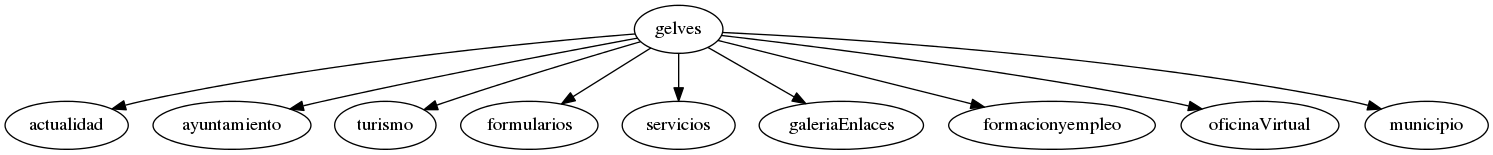
\includegraphics[scale=0.45]{trabajo_previo/Gelves.png}
\caption{Web de Gelves}
\end{subfigure}

\begin{subfigure}[b]{0.5\textwidth}
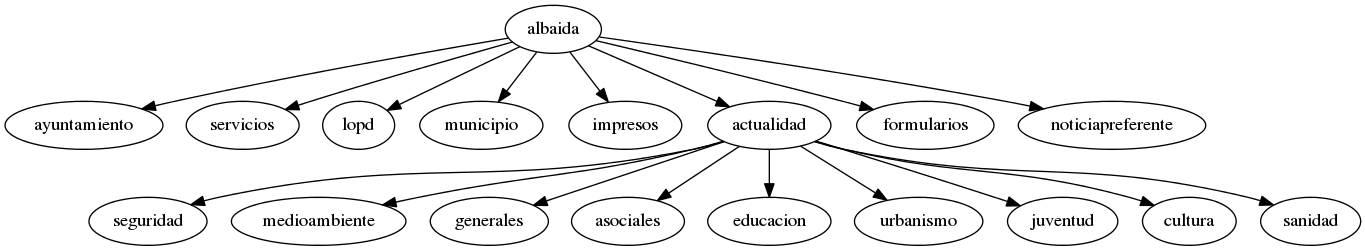
\includegraphics[scale=0.5]{trabajo_previo/Albaida_del_aljarafe.png}
\caption{Web de Albaida del Aljarafe}
\end{subfigure}
\caption{Grupos 1 y 4}
\label{fig:grupo14}
\end{sidewaysfigure}


\begin{sidewaysfigure}
\hspace*{-1cm}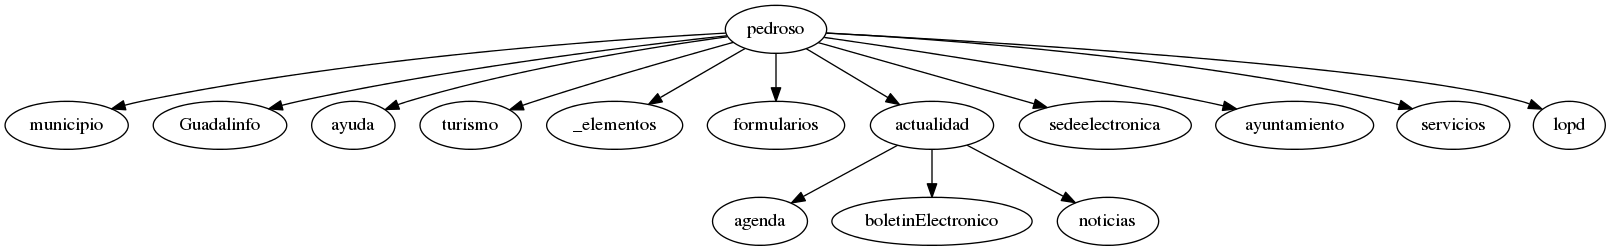
\includegraphics[scale=0.4]{trabajo_previo/El_pedroso.png}
\caption{Web de El Pedroso, Grupo 2}
\label{fig:grupo2}
\end{sidewaysfigure}
\begin{sidewaysfigure}


\begin{subfigure}[b]{0.5\textwidth}
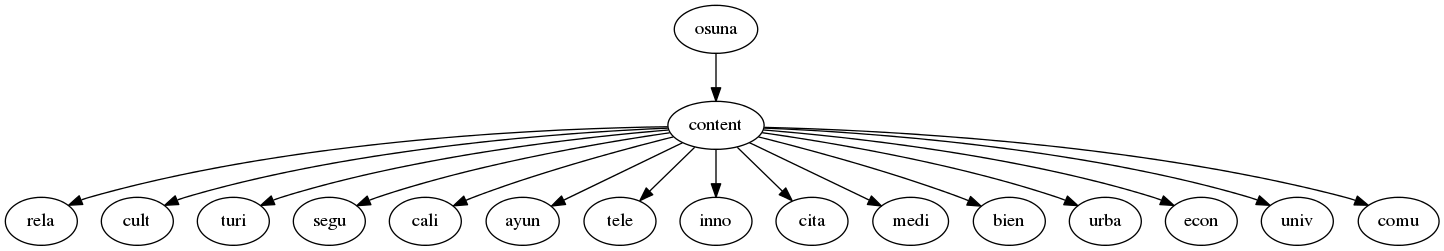
\includegraphics[scale=0.45]{trabajo_previo/Osuna.png}
\caption{Web de Osuna}
\end{subfigure}

\begin{subfigure}[b]{0.5\textwidth}
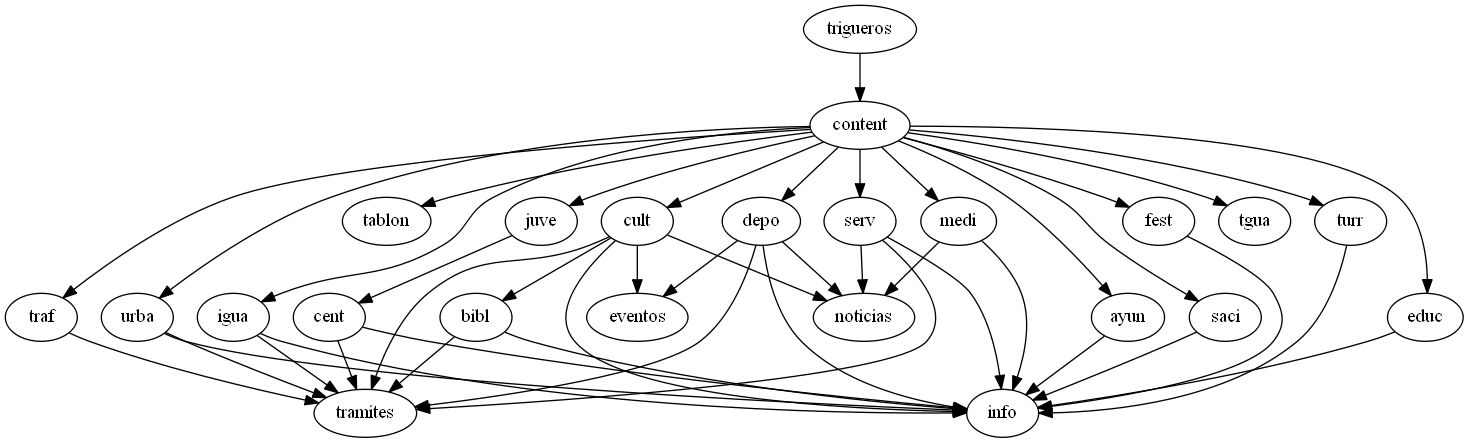
\includegraphics[scale=0.45]{trabajo_previo/Trigueros.png}
\caption{Web de Trigueros}
\end{subfigure}
\caption{Grupo 3}
\label{fig:grupo3}
\end{sidewaysfigure}
\begin{sidewaysfigure}

\begin{subfigure}[b]{0.5\textwidth}
\hspace*{-2cm}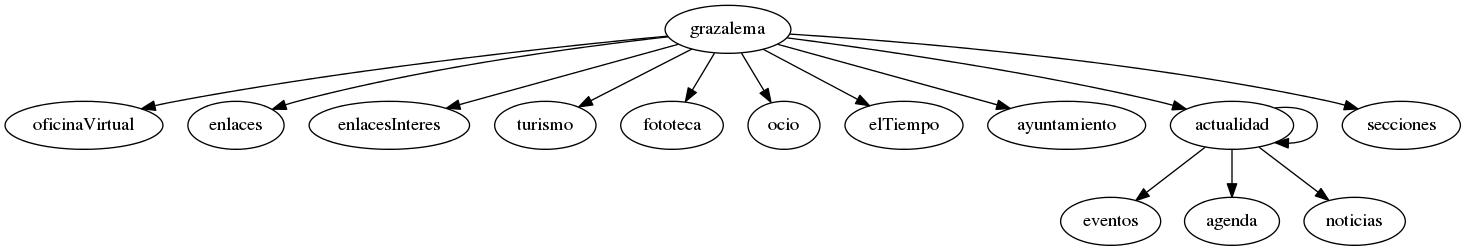
\includegraphics[scale=0.45]{trabajo_previo/Grazalema.png}
\caption{Web de Grazalema}
\end{subfigure}

\begin{subfigure}[b]{0.5\textwidth}
\hspace*{-1.6cm}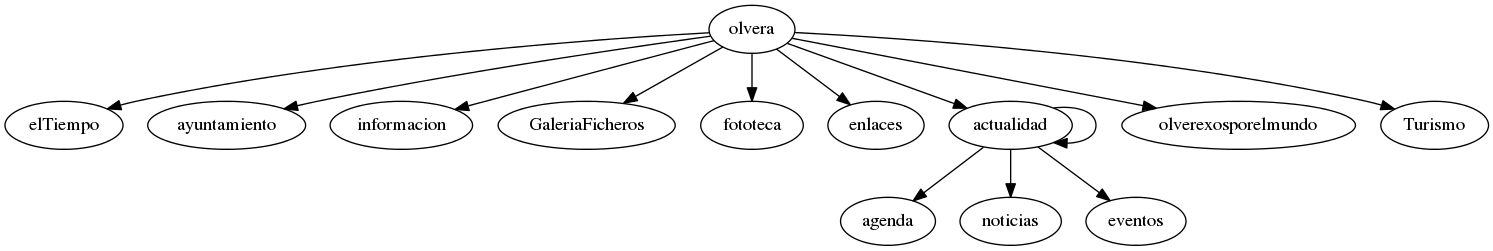
\includegraphics[scale=0.45]{trabajo_previo/Olvera.png}
\caption{Web de Olvera}
\end{subfigure}
\caption{Grupo 5}
\label{fig:grupo5}
\end{sidewaysfigure}

\subsection{Resultados}

Una vez podemos determinar a que grupo pertenece cada municipio, la figura \ref{fig:grupos} muestra la distribución de los datos:

\begin{figure}[h]
\centering
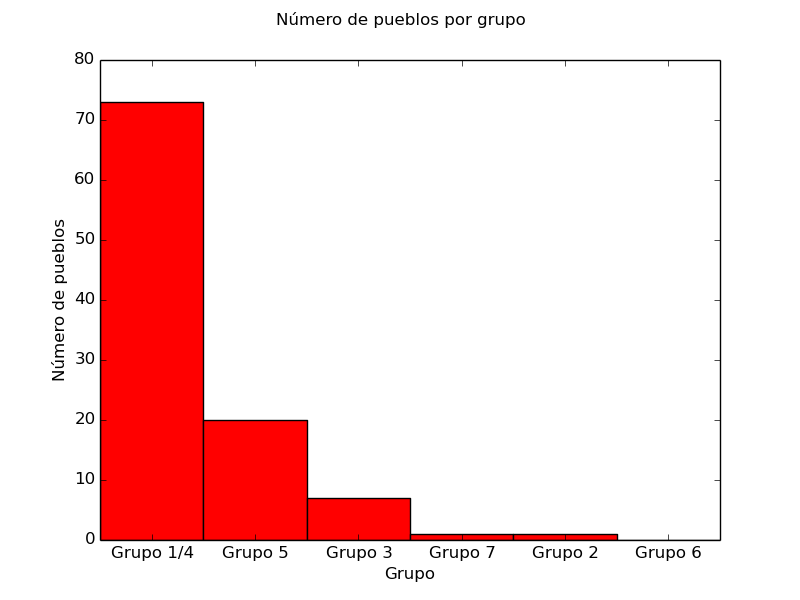
\includegraphics[scale=0.65]{trabajo_previo/histograma.png}
\caption{Municipios por grupos}
\label{fig:grupos}
\end{figure}
